
\documentclass[]{beamer}

\usepackage{graphicx}
\usepackage{tikz}
\usetikzlibrary{positioning}
% \usepackage[mode=buildnew]{standalone} % Allows inclusion of standalone files

\usepackage{caption}
\usepackage{subcaption}

% define a style for a tikz node with a smaller font size and texttt font
\tikzset{message/.style={font=\small\ttfamily}}


\usetheme{default} % Change "default" to a specific theme, e.g., "Madrid" or "Berlin"
\title{ORCA: Observability with Realtime Control and Aggregation}
\author[Left Text]{Ankush Jain}
\institute{CMU}
\date{\today}

\begin{document}

% \begin{frame}
%   \titlepage % Generates the title slide
% \end{frame}

\begin{frame}{Agenda 20250211: SQL/Arrow Integration Walkthrough}
	\begin{enumerate}
		\item Data structures, memory management
    \item Rust FFI and compilation
    \item Status: overlay bootstraps all topologies
      \begin{enumerate}
        \item Not thoroughly tested, Sheng discovered many bugs
        \item Getting robust over time
        \item TODO: remote failure handling
          % change text color below to light gray
        \item \textcolor{lightgray}{TODO (note for self): aggregator address exchange}
      \end{enumerate}
    \item Status: basic SQL works
      \begin{enumerate}
        \item One rank sends a table
        \item Aggregator saves it async and processes it
        \item Processed table forwarded to controller
      \end{enumerate}
	\end{enumerate}
\end{frame}

\begin{frame}{Previously: Topologies}
	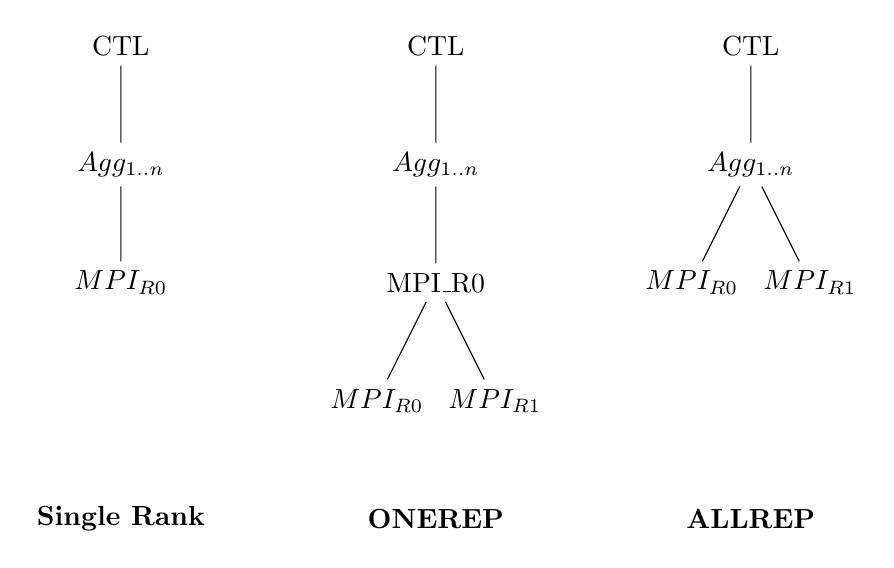
\begin{tikzpicture}
		% shift scope by 1cm xshift
		\begin{scope}[xshift=1cm]
			\node (a) {CTL}
			child { node (b) {$Agg_{1..n}$}
					child { node (c) {$MPI_{R0}$} }
				};
			\node at (0, -6) {\textbf{Single Rank}};
		\end{scope}

		\begin{scope}[xshift=5cm]
			\node (a) {CTL}
			child { node (b) {$Agg_{1..n}$}
					child {
							node (c) {MPI\_R0}  {
									child { node (d) {$MPI_{R0}$} }
									child { node (e) {$MPI_{R1}$} }
								}
						}
				};
			% add a text node LABEL at the bottom
			\node at (0, -6) {\textbf{ONEREP}};
		\end{scope}

		\begin{scope}[xshift=9cm]
			\node (a) {CTL} {
				child { node (b) {$Agg_{1..n}$}
						child { node (c) {$MPI_{R0}$} }
						child { node (d) {$MPI_{R1}$} }
					}
			};
			% add a text node LABEL at the bottom
			\node at (0, -6) {\textbf{ALLREP}};
		\end{scope}

	\end{tikzpicture}
\end{frame}

% add slide with table of contents
\begin{frame}{Outline}
  \begin{itemize}
    \item ProbeCollector API + SQL Demo
    \item Then Arrow Datatypes + Memory Management
    \item Then Rust integration/building
  \end{itemize}
\end{frame}


% add fragile to frame
\begin{frame}[fragile]{Arrow Datatypes}
  \begin{itemize}
    \item \verb|arrow::Array|: contiguous array, like C arrays
      \pause
    \item \verb|arrow::RecordBatch|: collection of arrays
      \pause
    \item \verb|vec<arrow::RecordBatch>|: collection of batches (table)
      \pause
      \begin{itemize}
        \item Concatenation of memory fragments
        \item \verb|ChunkedArray| and \verb|Table| are not used in datafusion
        \item \verb|Schema|: metadata about columns
        \item \verb|RecordBatch|: collection of N \verb|Array|s + one \verb|Schema|
      \end{itemize}
    \item \verb|arrow::Buffer|: contiguous memory
      \begin{itemize}
        \item \verb|arrow::ipc|: serialization/deserialization
        \item Conversion between types is zero-copy (not sure about serdes)
      \end{itemize}
      %\pause
  \end{itemize}
\end{frame}

\begin{frame}[fragile]{Arrow Memory Management}
  \begin{itemize}
    \item Fairly sophisticated, all structs are wrapped in \verb|std::shared_ptr| 
    \item Frees automatically when it goes out of scope
    \item Conversion between types has move semantics
    \item Move semantics provided even across language boundaries
      \begin{itemize}
        \item So if a Batch is sent from Cpp to Rust, zero-copy move to Rust
        \item Rust will free after usage
      \end{itemize}
  \end{itemize}
\end{frame}

\begin{frame}[fragile]{Arrow Data Generation}
  \begin{itemize}
    \item DataCollectors (our abstraction)
    \item A datacollector implements a schema
    \item Essentially a struct declaration with boilerplate
    \item Example schema: \verb|[timestep, timestamp, rank, probe_id, probe_val]|
  \end{itemize}
\end{frame}

\begin{frame}[fragile]{Rust + Datafusion}
  \begin{itemize}
    \item Currently only have single-node datafusion
    \begin{itemize}
      \item Essentially out-of-the-box datafusion
      \item (Distributed queries would be a lot more complicated)
    \end{itemize}
    \pause
    \item Opaque \verb|DfRustCtx| struct for datafusion context
    \pause
    \item C-level \verb|summarize(recordbatch, sqlquery)| API
    \pause
    \item Asynchronous C++ \verb|Executor| wraps Rust Context
  \end{itemize}
\end{frame}

\begin{frame}[fragile]{Rust Integration + Building}
  \begin{itemize}
    \item CMake calls Cargo to build \verb|rustcore|
    \begin{itemize}
      \item Cargo (Rust buildsystem) generates \verb|librustcore.a|
      \item Statically linked with the main binary
    \end{itemize}
    \pause
  \item We add \verb|cbindgen| to cargo to generate headers
  \item \verb|make rustgen| on the cpp side will invoke it
    \pause
  \item Generated headers are checked into the repo
  \end{itemize}
\end{frame}

% -- SEQ DIAG --
% \begin{frame}
% 	\begin{tikzpicture}[node distance=2cm]
%
% 		% Entities
% 		\node (MPI) [draw, rectangle] {MPI};
% 		\node (CTL) [right=4cm of MPI, draw, rectangle] {CTL};
% 		\node (AGG) [right=4cm of CTL, draw, rectangle] {AGG};
%
% 		% Messages
% 		\draw[->] (MPI) -- node[above] {Hello} (CTL);
% 		\draw[<-] (MPI) -- node[below] {Hello Back} (CTL);
%
% 		\draw[->] (MPI) -- node[above] {Hello} (AGG);
% 		\draw[<-] (MPI) -- node[below] {Hello Back} (AGG);
%
% 	\end{tikzpicture}
% \end{frame}
% -- SEQ DIAG --

\begin{frame}{Next Steps}
	\begin{itemize}
		\item Implement complete monitoring API (MPI-side, preload-derived)
      \begin{itemize}
        \item Sheng implementing a Probe ID directory
        \item Need mechanisms to declare schemas, enable/disable probes
        \item ProbeDataCollector: template for all data collectors
        \item Control + tuning: minor additions but may not be immediately necessary
      \end{itemize}
    \item Complete single-node aggregation
      \begin{itemize}
        \item Aggregator waits for N tables from all ranks
        \item Concatenates them and then processes them
      \end{itemize}
    \item Some realtime data visualization on controller
    \item Next: distributed queries

	\end{itemize}
\end{frame}

\end{document}
